In the past decade new video coding standards have achieved state-of-the-art coding performance. H.264/AVC typically requires 60\% or less of the bit rate compared to previous standars to achieve the same reconstruction quality \cite{H264_Overview}. In comparison, H.265/HEVC requires around 50\% less then H.264/AVC. Next, a short overview on both codecs is given.\\
\\
The H.264/AVC \cite{h264joint}, \cite{H264_Overview} video coding algorithm is depicted in block diagram \ref{h264}.

\begin{figure}[H]
\centerline{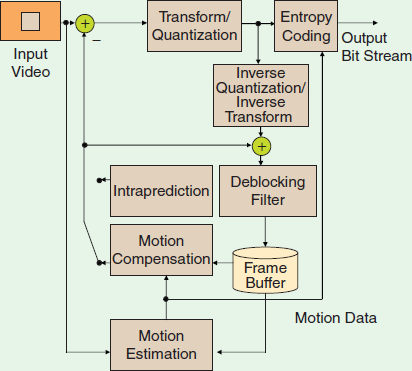
\includegraphics[scale=0.5]{pics/H264_Blockschaltbild}} % The bounding box is set manually in this example. Useful for some .pdf figures.
\caption{\label{h264}{\it H.264/AVC encoding algorithm (taken from \cite{Paper1})}}
\end{figure} % [width=5in,bb= 36 253 574 500]

It is designed on a block-based hybrid approach which has been a wide spread used approach for many video codecs. On the one hand it exploits spatial correlation between neighbouring pixels and on the other hand it uses the correlation between neighbouring pictures. This method has been used by many codecs before, but there are many highlights compared to previous standards like MPEG-2 \cite{MPEG2}, from which some are shown next.\\
Variable block-size motion compensation (VBSMC) is supported with different block sizes downto 4x4 for luma motion compensation blocks. H.264 also allows quarter-sample-accurate motion compensation. Most standards previous to H.264 only featured half-sample-accuracy.\\ The decoupling of referencing order from display order of images ensures that the flexibility of the encoder is only constraint to the memory. It is also possible to use all encoded pictures for further referencing, which isn't the case in other previous codecs.\\
Another important highlight is the in-loop deblocking filter, which filters the blocking artifacts that occur at block-based video coding algorithms. This filter is combined with the motion-compensation prediction loop to use the improvement in quality from the deblocking filter for better inter-prediction.\\
An additional feature from the H.263 codec was the entropy coding which is a standard feature in H.264. The CABAC (context-adaptive binary arithmetic coding) \cite{cabac} is a powerful entropy coding algorithm to gain further compression without loosing quality at all.\\
There are many more highlights of the H.264 codec that can't all be named in this article due to its size, but that can be found in \cite{H264_Overview}.\\
\\


The H.265/HEVC \cite{H265_Overview} block diagram is depicted in \ref{h265}. 


\begin{figure*}[ht]
\centerline{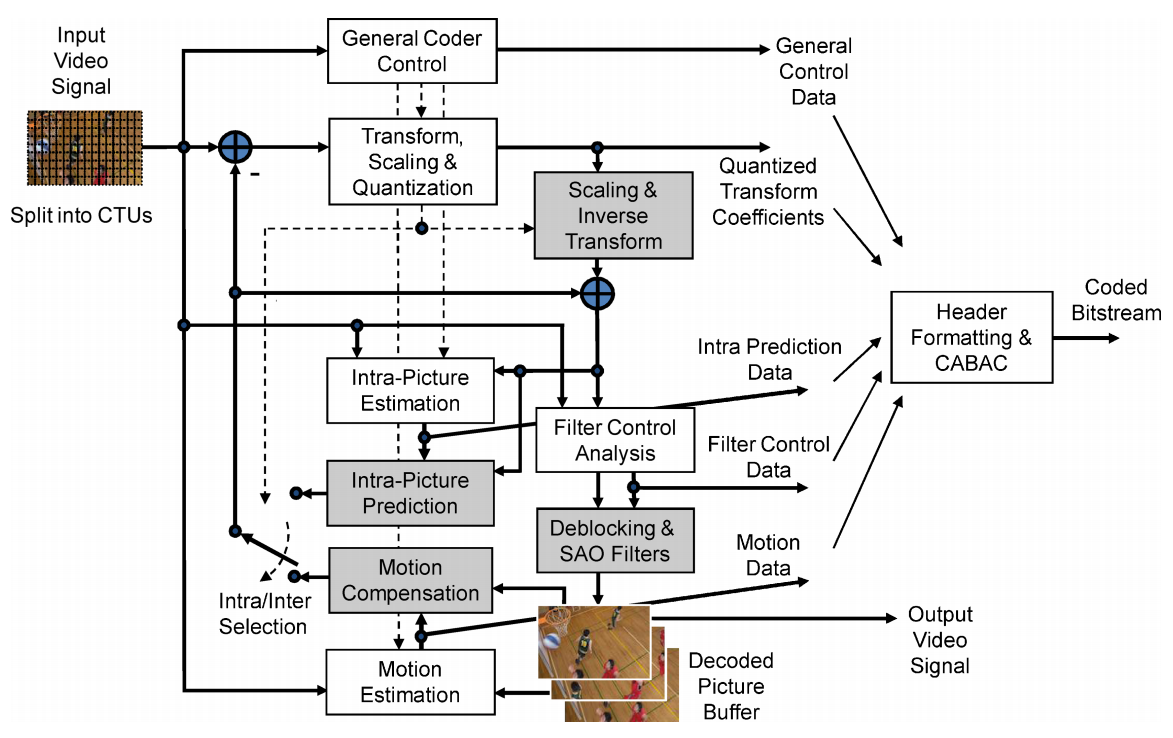
\includegraphics[scale=0.45]{pics/H265_Blockschaltbild}} % The bounding box is set manually in this example. Useful for some .pdf figures.
\caption{\label{h265}{\it H.265/HEVC encoding algorithm (taken from \cite{H265_Overview})}}
\end{figure*} % [width=5in,bb= 36 253 574 500]

The codec is very similar to H.264 but has some major improvements regarding parallelization and aims to reach the goal of having around half the size of an H.264 video while maintaining the same quality. Some of the many highlights are mentioned below.\\
\\
In H.265 a new structure for handling the macroblocks was introduced, the coding tree units (CTU). They basically replace the macroblocks from the H.264 codec. They are variable in size with a maximum of 64x64, for it is larger than the maximum macroblock size. They consist of luma coding tree blocks (CTB) and the corresponding chroma CTBs and can be partitioned into smaller blocks, called coding blocks (CB). 3 CBs form one coding unit (CU). This CTU/CTB structure allows the H.265 to be more flexible for inter and intra prediction of the blocks.\\
The H.265 codec also supports variable prediction block sizes from 64x64 down to 4x4 samples.\\
The deblocking filter and the entropy coder are still the same like in H.264, but with some improvements towards throughput speed and parallelism. Additionally to the deblocking filter a sample adaptive offset filter was added, which allows the image to be better reconstructed by applying another advanced filter after the deblocking filter. This filter improves the result significantly by just using a few percent more computation time.
